\section*{Introduction du chapitre}
L'\es n’est pas un concept construit par des chercheurs, mais une réalité économique. Elle ne s’est pas développée uniformément, mais en fonction des contextes politiques et économiques des différents pays. Une étude au niveau européen a montré que dans des pays voisins, l’\es était perçue et institutionnalisée de manière parfois très différente \parencite{monzon_campos2012social}. Dans des pays comme la France, où a émergée l’\es, mais aussi l’Espagne ou la Grèce, elle est reconnue par les pouvoirs publics et la communauté scientifique. D’autres États lui préfèrent d’autres concepts, comme celui de secteur non lucratif (\textit{non-profit sector}), d’organisations non gouvernementales, de tiers secteur ou encore d’entreprises sociales. C’est le cas par exemple en Allemagne, en Finlande ou aux Pays-Bas. Ces divergences ne sont pas seulement terminologiques, mais englobent chacune un périmètre distinct. L’approche de l’ES la plus large intègre les coopératives, mutuelles, associations, fondations et, souvent, des formes d’entreprises sociales. L’approche du secteur non lucratif, en revanche, exclut généralement les coopératives et mutuelles \parencite{laville2000leconomie}. Il existe en outre de nombreux statuts spécifiques à un pays, qui peuvent être intégrés dans le périmètre de l’\es (ex : les \cit{Centres d’Intégration Socio-Economique} en Pologne, ou les \cit{compagnies populaires} en Grèce). Le constat est similaire au niveau international. Les États-Unis ont majoritairement recours au concept de \citit{nonprofit sector} \parencite{hansmann1980role} et de \cit{tiers secteur} \parencite{salamon2016beyond}. En France comme au Canada, notamment au Québec en raison de leurs liens historiques, on parle d’ESS, mais avec la même confusion \parencite{levesque1999leconomie}. Ces divergences ont constitué un frein important à une conceptualisation claire et consensuelle du secteur. \\

En France, alors que les professionnels de l’\ess ont longtemps déploré un manque de reconnaissance et un cadre législatif insuffisant \parencite{vercamer2010leconomie}, la loi du 31 juillet 2014 a permis de moderniser l’approche de ce secteur. Elle établit clairement les critères d’appartenance à l’ESS et met en place un agrément \esus. L'article 1 adopte la définition suivante :

\begin{quotation}
    \textit{
    - L'économie sociale et solidaire est un mode d'entreprendre et de développement économique adapté à tous les domaines de l'activité humaine auquel adhèrent des personnes morales de droit privé qui remplissent les conditions cumulatives suivantes :
     \begin{enumerate}
     \item Un but poursuivi autre que le seul partage des bénéfices ;
     \item Une gouvernance démocratique, […]
     \item Une gestion conforme aux principes suivants :
      \begin{itemize}
      \item Les bénéfices sont majoritairement consacrés à l'objectif de maintien ou de développement de l'activité de l'entreprise ;
      \item Les réserves obligatoires constituées, impartageables, ne peuvent pas être distribuées. […]
      \end{itemize}
     \end{enumerate}}
\end{quotation}

Elle précise que l’\ess est composée des coopératives, des mutuelles, de fondations et d’associations, ainsi que de sociétés commerciales recherchant une utilité sociale et respectant des principes de gestion visant notamment à limiter la distribution des bénéfices. Il est ainsi précisé qu’au moins 70 \% du bénéfice doit être affecté au report du résultat ou aux réserves obligatoires. De plus, les opérations sur capital ne sont possibles que si elles sont indispensables à la continuité de l’activité. \\

L’ES se structure aussi autour de certains principes de fonctionnement auxquels adhèrent ses organisations. En 1980, le CNLAMCA (Comité National de Liaison des Activités Mutualistes Coopératives et Associatives) publie la \cit{charte de l’Économie Sociale} constituée de sept engagements des entreprises de l’ES. Ces principes ont été repris dans la \cit{Charte des principes de l’Économie Sociale} publiée par la Conférence Européenne des Coopératives, Sociétés Mutuelles, Associations et Fondations \parencite{monzon_campos2012social} :
\begin{quotation}
 \begin{itemize}
 \textit{
     \item The primacy of the individual and the social objective over capital
     \item Voluntary and open membership
     \item Democratic control by membership (does not concern foundations as they have no members)
     \item 	Combination of the interests of members/users and/or the general interest
     \item 	Defence and application of the principle of solidarity and responsibility
     \item 	Autonomous management and independence from public authorities
     \item 	Use of most of the surpluses to pursue sustainable development objectives, services of interest to members or the general interest.} \\
     \end{itemize}
\end{quotation}

Dans une première partie de ce chapitre, nous décrivons ce qu'est l'\ess sur le terrain en France. Ceci a pour objectif de mieux comprendre la complexité et la diversité de ce secteur. Nous rentrons ensuite en détail dans les perspectives théoriques fréquemment retenues. Enfin, nous introduisons le concept d'identité organisationnelle qui offre une perspective intéressante pour étudier les \eess.

\section{Des réalités diverses}

    Les principes présentés précédemment constituent le dénominateur commun d’une économie par ailleurs très diverse \parencite{mariaux2015leconomie}. L’\ess opère dans la grande majorité des secteurs d’activité. Selon l’INSEE\footnote{Chiffres INSEE, 2013}, son poids est particulièrement important dans les activités financières et l’assurance (30,8 \% de l’effectif salarié en France), dans l’enseignement (18,7 \%), la santé humaine (11,3 \%) et l’action sociale (60,9 \%). Elle représente aussi 41 \% de l’emploi dans le milieu des arts et du spectacle. Elle intervient également dans des secteurs comme l’industrie et la construction, l’agriculture ou encore le commerce, mais de façon beaucoup plus minoritaire (resp. 1,1 \%, 4,5 \% et 1,9 \%). L’\ess produit aujourd’hui environ 10 \% du PIB français. \\


    Décrire l’\ess par les principaux types d’organisations qui la composent tend à masquer à la fois sa diversité et sa complexité. La logique coopérative faisant partie de l’ADN de ce segment de l’économie, les organisations comme les individus engagés dans l’\ess s’organisent en réseaux, en fédérations, en collectifs, mènent des projets communs et s’inscrivent dans des démarches partenariales fortes. Tout comme les entreprises classiques, celles de l’\ess peuvent également constituer des groupes associatifs, mutualistes ou coopératifs.
    Avant de présenter les approches théoriques de l'ESS, cette section vise à donner un panorama des structures qui la constitue (au moins en France) et d'en illustrer la grande diversité. Quelques exemples sont donnés afin d’illustrer ces cas. Cette description met aussi en lumière la difficulté à distinguer nettement trois « segments » de l’économie (secteur public, secteur privé à but lucratif, \ess).


    \subsection{Les cinq familles de coopératives}

        Selon CoopFR, organisme représentatif du mouvement coopératif français , il faut distinguer cinq grandes familles de coopératives.
        \begin{itemize}
            \item Les coopératives d’entreprises, qui sont détenues par des entrepreneurs, commerçants ou artisans. On y retrouve notamment les coopératives agricoles, maritimes, ou encore les groupements de transporteurs. Exemple : la coopérative agricole UNEAL associe des producteurs céréaliers et animaliers et assure des activités de collecte des productions et de logistique.
            \item Les coopératives d’usagers, qui appartiennent à leurs clients. Elles intègrent notamment les coopératives scolaires et coopératives d’HLM. La coopérative \cit{La Louve}, supermarché participatif à Paris constitue un exemple d’une entreprise créée et détenue par ses clients. En outre, ce sont les clients membres qui font fonctionner l’entreprise en donnant bénévolement de leur temps.
            \item Les coopératives bancaires, également détenues par leurs clients, mais qui opèrent spécifiquement dans le domaine financier. Le Crédit Coopératif est un exemple d’une banque appartenant à ses clients. Il intègre une dimension solidaire dans l’ensemble de ses produits en donnant la possibilité de faire des dons ou de reverser une partie des intérêts à des associations.
            \item Les coopératives participatives qui associent au capital leurs salariés. On distinguera les \scop et les \cae. Créée en 2008, la \scop GreenBuro agit à la fois pour l’environnement et pour l’insertion, en proposant un service de gestion des déchets pour les entreprises et un effectif composé à moitié de salariés en insertion.
            \item Les coopératives multisociétariales qui intègrent au capital des parties prenantes multiples (salariés, clients, fournisseurs, collectivités…). Elles prennent la forme de \scic ou de \sce. Un exemple est la \scic Enercoop, fournisseur d’électricité exclusivement issue de sources d’énergies renouvelables. Sa gouvernance intègre 5 collèges : producteurs, consommateurs, salariés, partenaires, porteurs de projet et collectivités locales.

        \end{itemize}

    \subsection{Les mutuelles : deux cadres législatifs}
        Bien qu’elles opèrent dans un secteur d’activité précis, celui de la santé et de la prévoyance, et de manière assez similaire, les mutuelles dépendent de deux régimes juridiques différents. La loi du 31 juillet 2014 intègre ainsi à l’ESS les coopératives, mutuelles ou unions relevant du code de la mutualité et les sociétés d'assurance mutuelles relevant du code des assurances (Article 1).

    \subsection{Des associations de citoyens, d’entreprises ou d’acteurs publics}
        L’association constitue une forme juridique en tant que telle, réglementée par la loi du 1er juillet 1901 (on parle \cit{d’association loi 1901}). Différents types d’associations vont pourtant se distinguer, notamment par leurs adhérents. Les membres d’une association peuvent être des individus, particuliers ou professionnels, mais aussi des organisations privées ou publiques, appartenant ou non au champ de l’économie sociale.

        Ainsi, l’APGH, Association des Professeurs d’Histoire-Géographie, rassemble des membres individuels ayant une activité professionnelle précise (enseignants du secondaire et du supérieur) dans le but de permettre l’épanouissement « des élèves et des enseignants […] au sein de la République. » . En revanche, les adhérents de l’association AfricaFrance  sont des personnes morales (TPE, PME, grandes entreprises, collectivités). Leur ambition est de développer les échanges commerciaux entre la France et les pays du continent africain.  Contrairement à l’APGH qui constitue une démarche citoyenne, AfricaFrance a été créée à l’initiative de chefs d’États et s’inscrit donc dans une démarche de politique économique faisant intervenir des acteurs aussi bien publics que privés.

    \subsection{Fondations abritantes, abritées et fondations d’entreprises. }
        Selon l’article 18 de la loi du 23 juillet 1987, \citit{La fondation est l'acte par lequel une ou plusieurs personnes physiques ou morales décident l'affectation irrévocable de biens, droits ou ressources à la réalisation d'une œuvre d'intérêt général et à but non lucratif}. Une fondation peut être une personne morale ou bien être \cit{abritée} par une fondation dite \cit{abritante}  . Dans ce cas, elle dépend juridiquement de la fondation abritante, partage son objet, mais dispose toutefois d’une autonomie dans la réalisation de ses activités. La Fondation de France, qui supporte toutes les causes visant à \citit{construire un monde meilleur}  abrite ainsi 721 fondations œuvrant contre la précarité, pour la culture, l’environnement, l’éducation ou encore la recherche.

        La loi du 4 juillet 1990 donne un statut aux fondations d’entreprises, c’est-à-dire créées à l’initiative d’une ou plusieurs sociétés commerciales, et qui prennent le nom d’une de ces sociétés. Cet outil est utilisé par de nombreuses entreprises du secteur privé lucratif et leur permet de mettre en œuvre des activités de mécénat entrant dans le cadre de leur responsabilité sociale. ENGIE, entreprise cotée en bourse, a par exemple créée une fondation visant à œuvrer pour la solidarité et l’environnement, s’inscrivant dans le cadre de \citit{l’engagement social, sociétal et environnemental du Groupe ENGIE et de ses collaborateurs\footnote{\url{http://www.engie.com/engagements/solidarite/fondation/}}}.

    \subsection{Les PTCE}
      \label{ptce}
        Mis en place au cours des dernières années, les \ptce constituent une forme d'organisation nouvelle visant à répondre à des besoins économiques, organisationnels, sociaux et environnementaux sur des territoires donnés \parencite{le_labo_de_less2017enquete}.
       \citit{Les pôles territoriaux de coopération économique sont constitués par le regroupement sur un même territoire d'entreprises de l'économie sociale et solidaire, au sens de l'article 1\up{er} de la présente loi, qui s'associent à des entreprises, en lien avec des collectivités territoriales et leurs groupements, des centres de recherche, des établissements d'enseignement supérieur et de recherche, des organismes de formation ou toute autre personne physique ou morale pour mettre en œuvre une stratégie commune et continue de mutualisation, de coopération ou de partenariat au service de projets économiques et sociaux innovants, socialement ou technologiquement, et porteurs d'un développement local durable.} \parencite[][article 9]{noauthor2014loi}
        Le \ptce ne constitue donc pas une forme juridique d'organisation, mais plutôt une démarche (qui s'appuie juridiquement sur une structure de l'ESS, majoritairement des associations ou des \scic). Selon une étude de \textcite{le_labo_de_less2017enquete}, ces pôles répondent à quatre catégories de besoins:
        \begin{itemize}
            \item des besoins économiques (coopération économique ; débouchés économiques ; renforcement de l'offre sociale, écologique ou économique ; accès à des compétences et des moyens matériels) ;
            \item des besoins organisationnels (organisation d'un projet territorial ; mutualisation des compétences, des lieux et des moyens ; structuration des activités déjà existantes) ;
            \item des besoins sociaux (développement d'un maillage d'acteurs ; création de lien social ; accompagnement d'un public spécifique ; \rse) ;
            \item des besoins environnementaux (logement et gestion des déchets ; préservation d'espaces naturels ; maîtrise et valorisation de l'énergie ; lutte contre la pollution). \\
        \end{itemize}
        L'étude souligne la primauté donnée aux besoins économiques et organisationnels par rapport aux besoins sociaux, et à plus forte raison aux besoins écologiques.


    \subsection{Les groupes d'économie sociale}
        Tout comme les entreprises du secteur privé classique s'organisent en groupes pouvant avoir une dimension nationale voire multinationale, les entreprises de l'\ess constituent parfois des groupes de taille importante. Le Groupe SOS, principal groupe d'\ess en France, constitue un excellent exemple d'un tel regroupement d'entreprises ayant des statuts différents. Il rassemble de nombreuses entreprises agissant dans les domaines de la jeunesse, l'emploi, la solidarité, la santé et les séniors. Le groupe est contrôlé par quatre associations fondatrices qui détiennent le contrôle exclusif de toutes les sociétés du groupe, garantissant ainsi la non-lucrativité puisque l'actionnariat individuel est impossible. La gestion du groupe est assurée par un directoire sous le contrôle des conseils d'administration des quatre associations fondatrices. \\

        D'autres montages plus complexes peuvent être observés, notamment dans les banques coopératives, ce qui amène parfois à s'interroger sur leur éloignement de l'identité originelle de l'\ess \parencite{bidet2003insoutenable}. Le groupe Crédit Agricole communique fréquemment sur son identité coopérative, issue du réseau des Caisses Régionales, alors même que la holding est une société cotée qui fait partie de l'indice CAC40.

    \subsection{Les fédérations}

        L'\ess s'organise également autour de nombreux organismes fédérateurs. Ces groupements garantissent la visibilité et la défense des intérêts des organisations. Elle peuvent prendre différentes formes (syndicats, associations) et s'organiser par secteur d'activité (ex : France Nature Environnement fédère des associations à visée écologique) ou par format d'organisations (ex : CoopFR fédère un grand nombre de coopératives dans tous les domaines).

        \begin{center}
            ***
        \end{center}



    Le seul cas de la France suffit à illustrer la diversité et la complexité de l'ESS. Il va de soit que les formes d'organisations évoquées ici ont des missions et des pratiques diverses, parfois très éloignées les unes des autres. C'est là un enjeu majeur de ce secteur, qui souffre de son manque de lisibilité et donc de visibilité \parencite{vercamer2010leconomie, davister2006gestion, monzon_campos2012social, huet2007pouvoir}. On parle pourtant - peut être abusivement - de \cit{secteur} de l'ESS. \textbf{Qu'est ce qui unit ces structures au sein d'un même ensemble ? Peut-on étudier de manière globale un champ d'entreprises aussi large ?} Dans la suite de ce chapitre, nous exposons différentes approches théoriques de l'\ess (ou concepts proches) et introduisons le concept d'identité organisationnelle qui permet de mettre en lumière des spécificités de ce segment de l'économie.

    \section{Des perspectives parfois contradictoires }

        L'ESS, souvent présentée comme un segment de l'économie, un \cit{mode d'entreprendre}, est aussi abordée sous l'angle de son lien avec la sphère sociale et politique. Dans cette perspective, elle associe économie et démocratie. Afin d'appréhender les différentes facettes de l'ESS, nous présentons dans cette section des approches économiques, gestionnaires et sociologiques. Dans un premier temps, l'ESS est perçue comme un « tiers secteur » qui vient compléter le rôle de l'État et du marché. Ensuite, nous discutons d'une perspective plus récente dans laquelle l'ESS constitue une vision sociale, éthique de l'entreprise. Enfin, un détour par la sociologie et l'économie politique nous permet d'envisager l'ESS comme une alternative au système économique dominant, à savoir le modèle capitaliste et l'idéologie néo-libérale.

        \subsection{Un tiers secteur }
            L'ESS est encore fréquemment approchée comme un \cit{tiers secteur}, c'est-à-dire comme ce qui n'est ni la sphère publique, ni l'économie capitaliste. Comme le suggère \textcite{draperi2015leconomie}, nous distinguons ici l'économie capitaliste de l'économie marchande ou de marché. L'économie marchande renvoie à \citit{l'économie dans laquelle la distribution des biens et services est confiée prioritairement au marché} \parencite{laville2000leconomie}. De nombreuses entreprises de l'ESS s'inscrivent dans ce mode de fonctionnement, mais se distinguent par la recherche d'un intérêt collectif. Pour Draperi, l'économie capitaliste désigne une économie marchande qui fait abstraction du lien social et dans laquelle la seule finalité est la rémunération du capital. La différence entre économie capitaliste et économie marchande réside donc dans la propriété des organisations davantage que dans les mécanismes économiques mobilisés. \\

            Au sein du tiers secteur, les organisations à but non lucratifs (\textit{nonprofit} ou \textit{voluntary organizations}) recueillent la plus grande attention des chercheurs. Depuis l'article fondateur de Hansmann (1980), la littérature s'intéresse en premier lieu aux fondements de ces organisations. Deux théories expliquent leur émergence et leur développement. La première repose essentiellement sur des aspects économiques. Elle est basée sur l'idée que le secteur non lucratif répond à des défaillances de marché \parencite{hansmann1980role} ou des défaillances gouvernementales \parencite{weisbrod1994nonprofit}. Les défaillances de marché se produisent dans des situations où le libre échange échoue à allouer de manière optimale les ressources. Elles sont généralement liées à l'existence de biens publics,  d'externalités positives ou négatives, ou d'asymétrie d'information. Lorsqu'un bien est public, ou lorsqu'une externalité positive est dégagée, l'entreprise rencontre des difficultés à être correctement rémunérée pour sa production : elle est donc peu incitée à investir sur ce marché, même lorsqu'il répond à une réelle demande de la société. Inversement, une externalité négative a un impact social qui n'est pas supporté par l'entreprise. Elle n'est donc pas incitée à réduire cette externalité. L'asymétrie d'information est une autre situation dans laquelle le marché peut se montrer sous-optimal : dans une situation où les deux parties d'un échange n'ont pas le même niveau d'information, l'un des acteurs économiques peut abuser de sa position et profiter de son avantage pour établir le prix d'un bien à un prix trop élevé ou trop faible. Les défaillances gouvernementales désignent quant à elles des situations où l'action des décideurs publics répond à une logique électorale plutôt qu'à la poursuite de ce qui est réellement l'intérêt public. \\

            En d’autres termes, cette économie existe pour correspondre à des situations qui ne sont prises en compte ni par le marché, faute de rentabilité, ni par l’État, faute d’intérêt politique (par exemple, répondre aux besoins d’une population très minoritaire). Ainsi, les associations endossent fréquemment un rôle de service public, se substituant à l’État défaillant. La résolution de ces échecs s’appuie sur le principe de non distribution des profits. Celui-ci est au cœur de la définition donnée par Hansmann :
            \begin{quotation}
            \citit{A nonprofit organization is, in essence, an organization that is barred from distributing its net earnings, if any, to individuals who exercise control over it, such as members, officers, directors, or trustees.} (p.838)
            \end{quotation}
             La non-distribution permet  au secteur non lucratif d’être jugé plus \cit{digne de confiance}. Par exemple, dans le cas d'une asymétrie d’information, l'entreprise libérale est incitée à dissimuler la qualité réelle d'un bien ou service pour proposer un prix supérieur à sa valeur. Au contraire, une entreprise non lucrative n’a pas cette incitation et peut fixer un prix plus juste. \\

            L’approche concurrente de cette théorie, portée par \textcite{rose-ackerman1996altruism}, se situe \cit{du côté de l’offre} et donne une place centrale aux valeurs. Elle propose que le secteur non lucratif n’existe pas seulement en raison d’une situation donnée du marché, mais aussi par une volonté de certaines personnes, des \cit{idéologues}, de promouvoir des croyances ou des convictions. Ces personnes entreprennent ou s’engagent dans le secteur non lucratif car il leur laisse plus de liberté pour exprimer ces convictions. Cette dimension idéologique peut en outre constituer un avantage compétitif par rapport à d’autres organisations concurrentes, en attirant un public partageant les mêmes valeurs, convictions ou croyances. Cette vision est partagée par des auteurs comme \textcite[][p.137]{rothschild2006centrality} : \citit{nonprofit organizations, by way of their very existence and practices, convey a public statement of what their members see as a better, more caring, or more just world.} Cependant, ceci ne doit pas conduire à une vision idéaliste de l’ESS qui la réduirait à \citit{une vision angélique, un utopisme} \parencite{laville2017conference}.\\

            Dans d’autres contextes, comme en Europe, au Québec ou en Amérique du Sud, l’ESS est appréhendée de façon plus large, incluant notamment les coopératives et les mutuelles. Celles-ci peuvent prendre des formes plus proches du secteur classique, à travers des statuts de sociétés de capitaux et une possible distribution d’une partie des profits, et constituent donc un champ d’étude distinct dans l’approche américaine. Toutefois, leur finalité et leurs modes de fonctionnement les rapprochent de l’ESS. Il en résulte une relative confusion dans la littérature et dans la terminologie utilisée. Un article de \textcite{salamon2016beyond}, et les réactions qu’il a suscité \parencite{defourny2016voluntas} ont permis une clarification du concept de \cit{tiers secteur}. Les auteurs font le triple constat d’un manque de clarté dans ses frontières, d’une hétérogénéité des termes employés pour s’y référer et du manque de visibilité dans les comptabilités nationales qui en résulte. L’étude aboutit à une définition basée sur cinq critères :
            \begin{quotation}
                \citit{
                    An institutional unit—whether a NPO, an association, a cooperative, a mutual, a social enterprise, or any other type of institutional entity in a country – must meet all five of these features to be considered ‘‘in-scope’’ of the third, or TSE, sector.
                	 In particular, to be considered part of the TSE sector, entities must be
                    \begin{itemize}
                        \item Organizations, whether formal or informal;
                        \item Private;
                        \item Self-governed;
                        \item Non-compulsory; and
                        \item Totally or significantly limited from distributing any surplus they earn to investors, members, or other stakeholders.
                    \end{itemize}
                } (p.19)
            \end{quotation}


            Conceptualisé ainsi, le tiers secteur intègre des composantes fortement hétérogènes : organisations à but non lucratif, mutuelles, coopératives, mais aussi les actions humaines hors d’un cadre organisationnel. Ces dernières renvoient au concept de \cit{société civile} ou de \cit{sphère publique} et incluent  \citit{the participation in demonstrations, other forms of political action, as well as other activities undertaken without pay for the benefit of one’s community or other persons beyond one’s household or family} \parencite{salamon2016beyond}. La définition inclut également les entreprises sociales, ici appréhendées comme des sociétés de marché adoptant une mission sociale. Il faut toutefois noter que la littérature reprend ce terme pour désigner des réalités bien différentes, allant d’un secteur non lucratif qui obtient une partie de ses revenus sur le marché à des entreprises capitalistes ayant une mission sociale combinée à la recherche de profit. Cette confusion est également observable dans la pratique, comme l’illustre en France le \mouves qui regroupe des sociétés commerciales, mais aussi des associations et des coopératives. Alors que la loi sur l’ESS de 2014 inclut de fait toutes les entreprises ayant une forme associative, coopérative ou mutualiste, cette définition théorique ajoute la contrainte d’un respect de critères normatifs. Le périmètre de l’ESS est donc restreint dans cette perspective.  \\

            La figure \ref{fig:tierssecteur} présente une synthèse des différentes composantes de l’ESS dans une perspective de tiers secteur. Dans l’approche institutionnelle française de l’ESS, les actions humaines individuelles ne sont pas prises en compte : l’ESS est exclusivement définie comme un ensemble d’entreprises.

             \begin{figure}[ht]
                 \centering
                 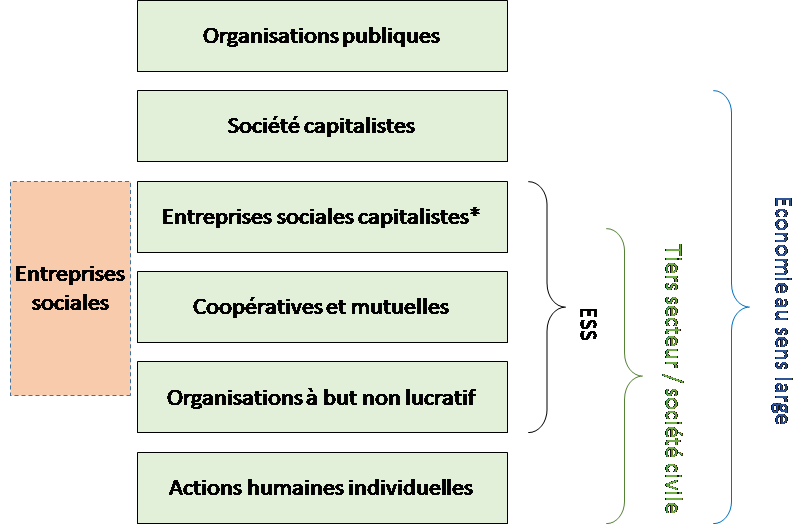
\includegraphics[width= 0.8\linewidth]{fig/tierssecteur.png}
                 \caption{L'ESS et le tiers-secteur}
                 \label{fig:tierssecteur}
             \end{figure}

            Si les auteurs ont salué la clarification apportée par \textcite{salamon2016beyond}, ils soulignent néanmoins que la question des frontières avec le secteur public et le marché n’est pas résolue et pose des problèmes d’opérationnalisation. En particulier, la question de la part des profits qui peut être distribuée reste à éclaircir \parencite{defourny2016voluntas}. Une autre critique de cette approche porte sur la terminologie, qui cantonne l’\ess à \cit{ce qu’il reste après l’État et le marché} et donc à négliger sa véritable place dans l’économie. L'\ess devient alors une composante de l"économie classique, une \citit{voiture balai} pour les personnes n'ayant pas trouvé leur place dans le système dominant \parencite{laville2011agir}. Cependant, un grand mérite de cette approche est d’être applicable au-delà des spécificités nationales et donc de rendre du compte du caractère universel de l’\ess \parencite{draperi2015leconomie}.


        \subsection{Un capitalisme social}

            L’ESS est souvent présentée comme une \cit{autre économie}, une \cit{économie alternative}, c’est-à-dire une alternative au système économique dominant. Elle s’inscrit alors dans une volonté de faire autrement, de proposer des schémas nouveaux qui remettent l’humain au cœur des activités économiques. Cependant, on observe un rapprochement récent entre l’\ess et le système capitaliste, faisant apparaître la première comme un fragment du système dominant qui adopterait une dimension sociale. Deux phénomènes mis en lumière dans la littérature nous semblent particulièrement bien éclairer cette évolution : l’émergence de l’entreprise sociale et la tendance croissante à l’adoption de logiques d’affaires dans l’ESS. \\

            L’entrepreneuriat social, concept issu du terrain, a donné lieu à une abondance de travaux au cours des dernières décennies. Il a donné naissance à plusieurs écoles adoptant des approches différentes du phénomène, allant des activités marchandes déployées par le secteur non lucratif jusqu’à l’intégration d’une mission sociale dans l’objet des sociétés capitalistes \parencite{defourny2011approches, petrella2014social}. L’école américaine des ressources marchandes met l’accent sur l’existence de ressources marchandes et de pratiques managériales issues du secteur privé classique. Les entreprises sociales sont d’abord définies comme des entreprises du secteur non lucratif qui déploient des activités économiques marchandes pour diversifier leurs sources de revenus. Une approche plus récente élargit le spectre à des entreprises à but lucratif dès lors que les ressources marchandes sont en partie mobilisées en vue d’une finalité sociale. Un cas particulier de cette école est celui du \textit{Social Business} popularisé par le prix Nobel de la paix Muhammad Yunus \parencite{yunus2010building, yunus2010building-1}. Ces entreprises ont une finalité sociale dont le coût est financé exclusivement par des ressources marchandes, selon la logique \citit{no profit, no loss}. Pour s’extraire du débat sur la lucrativité ou non des entreprises sociales,  l’école de l’Innovation Sociale se focalise non pas sur les ressources et leur usage, mais sur l’impact social et sur la nature de l’innovation qui génère cet impact. Cette logique est parfaitement résumée par le titre d’un article de \textcite{dees2003social} : \citit{Social Entrepreneurship is About Innovation and Impact, Not Income}. Au cœur de cette réflexion se situe l’entrepreneur (et non le collectif), moteur de l’innovation sociale. Enfin, \textcite{defourny2011approches} soulignent la spécificité de l’approche européenne, portée par l’EMES, qui s’appuie sur un idéal type basé sur neuf critères, relatifs aux dimensions économiques, sociales et de gouvernance de l’entreprise sociale. Les entreprises sociales ne sont donc pas définies strictement, mais doivent se rapprocher de cet idéal type. Dans la loi française, depuis 2014, le périmètre de l’ESS intègre des sociétés commerciales qui poursuivent une mission sociale. Elles doivent également respecter certaines règles de gestion portant sur la distribution des bénéfices, l’échelle des salaires ou encore la gouvernance et la démocratie d’entreprise. L’appartenance à l’ESS est formalisée par l’obtention d’un agrément (\esus). \\

            Un point commun des différentes approches de l’entreprise est de s’appuyer sur les schémas classiques de l’entreprise : que le profit soit possible ou non, les procédés managériaux et organisationnels sont ceux des entreprises capitalistes. Il ne s’agit pas du tout ici de remettre en cause le système dominant, mais au contraire de mobiliser ce qui a fait son succès, à savoir l’efficacité économique, pour résoudre les problèmes sociaux. Une forme d’économie sociale se développe donc au sein même du système économique dominant. Yunus propose ainsi un \citit{nouveau capitalisme}, c'est-à-dire un capitalisme qui ne serait pas orienté vers le profit mais vers une mission sociale, mais qui appliquerait les mêmes règles que le marché. Pour lui, les entreprises sociales sont en concurrence directe avec les entreprises de marché et doivent donc appliquer les mêmes règles et les mêmes modes de fonctionnement. Seule la finalité est différente. C’est la raison pour laquelle certains penseurs de l’ESS comme \textcite{draperi2015leconomie} contestent l’appartenance des entreprises sociales à l’ESS. \\

            Au-delà des entreprises sociales, l’ESS dans son ensemble est de plus en plus poussée à adopter un fonctionnement \citit{Business-like}  \parencite{dart2004being} qu’on pourrait traduire par \citit{ des logiques d’affaires}. Dans une récente revue de littérature, \textcite{maier2016nonprofit} recensent plusieurs raisons à ce phénomène déjà largement documenté, particulièrement pour le secteur non lucratif. Les premières raisons sont d’ordre stratégique et sont basées sur la rationalité économique. Faisant face à une concurrence croissante avec le secteur privé classique, ou au sein même de l’ESS, les entreprises cherchent à assurer leur indépendance et leur pérennité en s’appuyant sur des ressources de marché. Ceci est renforcé par la raréfaction des financements publics ou privés. En outre, les donateurs et partenaires privés ou publics, parties prenantes de la stratégie des entreprises de l’ESS, sont porteurs d’exigences en termes de performance et promeuvent l’application d’une logique d’affaires. Par ailleurs, ce changement est soutenu par la large prédominance de l’idéologie libérale au niveau international. S’inscrire dans ce système dont les codes sont omniprésents dans les sphères sociale, politique et économique devient un enjeu en termes de légitimité. Or celle-ci constitue une \citit{ressource opérationnelle} \parencite{suchman1995managing} et constitue un facteur indispensable de la pérennité des entreprises. La théorie institutionnelle souligne alors le rôle des isomorphismes : pour se légitimer, une entreprise cherche à ressembler à celles qui sont déjà légitimes, en reprenant les éléments qui les caractérisent, notamment les éléments symboliques comme les mythes, les symboles ou le vocabulaire \parencite{dimaggio2010iron, meyer1977institutionalized}. Or, comme le souligne \textcite{dart2004legitimacy}, le système économique basé sur le marché est devenu largement dominant, et donc plus légitime. L’ESS peut donc se légitimer en reproduisant ses pratiques :
            \begin{quotation}
                \citit{If business values, business models, and business language have become dominant and are the sociocultural environment’s preferred modes of problem solving and preferred structures of organizing, then it follows that even social-sector organizations can be accorded legitimacy by adopting the language, goals, and structures of this ideologically ascendant form.} (p.419)
            \end{quotation}

            En France, où l’ESS représente une part significative de l’économie et où le secteur associatif est fortement ancré, cette perspective d’un \cit{capitalisme social} est perceptible, comme l’illustrent quelques exemples symboliques. Le fondateur et dirigeant du plus grand groupe français d’économie sociale, Jean-Marc Borello a ainsi publié un ouvrage intitulé \citit{Pour un capitalisme d’intérêt général}. Plus récemment, le gouvernement a lancé \citit{l’initiative French Impact} qui vise à \citit{fédérer et valoriser la diversité des acteurs de l’innovation sociale} \parencite{ministere_de_leducation_nationale2018lancement}. L’ESS, ainsi intégrée dans un ensemble plus large autour d’un label et d’un objectif \cit{d’impact}, voit sa spécificité par rapport au reste de l’économie effacée. A tel point que le média Novethic suggère d’abonner l’expression \cit{économie sociale} au profit du \cit{French Impact} \parencite{alvarez2018ne}.

            Les études empiriques mettent en lumière des effets positifs de ces logiques d’affaires sur la performance et l’obtention de ressources humaines et financières. Elles semblent aussi aboutir à davantage d’innovations. Toutefois certains auteurs s’inquiètent de possibles dérives \parencite{maier2016nonprofit} et de la perte de l’identité des organisations \parencite[p. 134]{laville2016economie}. Le risque pour les entreprises est la focalisation sur la gestion et la performance, sur le marché et les clients, et la perte de vue des enjeux sociaux initialement adressés. Comment acquérir des ressources commerciales si les bénéficiaires initiaux sont justement insolvables ? La question se pose de l’équilibre entre les activités génératrices de ressources et les activités génératrice d’impact social.

            Pour certains auteurs, l’ESS est aussi porteuse d’une autre mission, celle de mettre la démocratie au cœur de l’économie. Or, l’économie néo-libérale serait précisément incompatible avec la démocratie \parencite{defalvard2016leconomie}. Ceci amène à une autre perspective de l’ESS, qui ne viserait pas seulement à résoudre des problèmes au niveau micro-économique, mais à porter un véritablement changement de société.

        \subsection{Une économie transformatrice }

            Plusieurs auteurs dans le champ du management comme de l’économie politique ou de la sociologie soulignent le rôle politique de l’ESS et sa mission démocratique. Cette dimension fondatrice de l’économie sociale n’a pourtant pas toujours occupé une place centrale. La perspective historique  proposée par \textcite{chanial2002leconomie} permet de comprendre l’articulation entre économie sociale, économie solidaire et démocratie. Au \siecle{19} siècle, la charité est individuelle et elle est utilisée comme un outil de contrôle par le système libéral pour maintenir la paix sociale. Elle n’a pas de volonté d’émancipation des pauvres, mais vise au contraire à créer des liens de dépendance. A cette vision, les associations opposent une « solidarité démocratique » reposant sur l’action collective. Dans cette approche, la solidarité est réciproque, chacun ayant une dette envers la société. Pour \textcite{laville2016economie}, l’associationnisme redonne alors sa place à la démocratie à travers \citit{l’expérience sociale et l’inflexion des politiques publiques} (p. 74). Comme l’expliquent \textcite{chanial2002leconomie}, le \siecle{20} siècle est marqué par des législations qui viennent scinder l’économie sociale en associations, coopératives et mutuelles, rompant ainsi sa dynamique sectorielle. Les coopératives se sont ancrées dans des logiques de marché quand les mutuelles et associations ont adopté un rôle complémentaire par rapport à l’État. A partir des années 1960, à travers différents mouvements sociaux et face à l’incapacité de l’État à pallier les failles du marché, renaît une économie solidaire porteuse d’une vision transformatrice de la société. Des initiatives émergent qui \citit{mettent l’accent sur le modèle de développement et sur la participation citoyenne.} (p. 19). Alors que l’économie sociale repose sur les formes de propriété, l’économie solidaire valorise une économie plurielle, associant les mécanismes de marché, de réciprocité et de redistribution. Cette perspective trouve ses racines dans les travaux de Karl Polanyi \parencite{servet2007principe, polanyi1944great}, qui introduit le concept d'économie \cit{encastrée} dans les structures sociales. Pour lui, l'approche libérale qui cherche à extraire complètement le système économique des relations sociales est vouée à l'échec, et une économie autonome, désencastrée, ne pourrait aboutir qu'à la destruction de la société \parencite{block2003karl, valensi1980karl}. \\

            Pour \textcite{defalvard2016leconomie}, l'\ess doit jouer un rôle politique pour faire face aux dérives du néolibéralisme. Selon lui, ce système se distingue du libéralisme originel par l’absence de fondement éthique (seule compte l’efficacité), l’absence d’intérêt réciproque, puisque seul compte l’intérêt individuel, et la primauté de la finalité monétaire (par opposition à l’utilité des biens acquis). A cette \cit{théorie du marché}, s’oppose une \cit{théorie des communs}. Pour l’auteur, l’ESS se distingue donc par sa capacité à recréer du commun, à constituer une alternative économique \cit{en commun} au système néo-libéral. Ceci n’exclut nullement l’échange marchand, mais cet échange s’effectue dans un rapport au marché différent de celui capitalisme, en ceci qu’il vise à renforcer le lien social plutôt qu’à le détruire, en adoptant un autre rapport au  développement et au territoire \parencite{draperi2015leconomie}.  Ainsi, pour \textcite[][p.64]{laville2016economie}, \citit{l’activité économique facilite l’émergence de l’expression politique} : elle permet aux individus de construire collectivement des solutions à leurs problèmes. L’ESS ne doit donc pas être vue seulement sous l’angle de l’économie capitaliste, mais aussi dans une perspective démocratique, comme le suggère \textcite{eikenberry2009refusing} :
            \begin{quotation}
                \citit{I suggest that, as an alternative to market-based discourse, nonprofit and voluntary organizations should focus their activities in a number of directions: on getting more people of diverse backgrounds to participate in organizational and societal governance, on making this participation meaningful in the sense of emphasizing relationships and engaging individuals “routinely in civic relationships over time” (Lichterman, 2006, p. 535), and on providing equal opportunities for members to participate in agenda setting, deliberation, and decision making.}
            \end{quotation}

            Pour l’auteure, ceci est incompatible avec une logique d’affaires, ancrée dans une logique d’intérêt individuel. Cette idée est partagée par \textcite{laville2011agir}, qui, s'appuyant sur les travaux d'Habermas, doute de la compabilité entre le capitalisme et la démocratie.
            En revanche, \textcite{dodge2016nonprofits} contestent la dimension a priori démocratique de l’ESS, ses organisations pouvant porter des pratiques et des valeurs contraires à celle de la démocratie. Sa place \citit{d’école de la démocratie} résulte nécessairement d’une démarche délibérée et active. Il convient donc d’écarter une vision idéaliste de l’ESS et des associations \parencite[][p. 26]{laville2016economie}. \textcite{mccambridge2004underestimating} insiste sur le rôle des organes de gouvernance des entreprises. Pour elle, l’ESS doit constituer un modèle de société et de démocratie. Elle a pour rôle d’amener les individus à participer à la vie civile et politique, rôle qui relève de la responsabilité du conseil d’administration. Ceci renvoie à un vaste champ de littérature sur la gouvernance de l’ESS et sur le rôle de cette instance \parencite{brown2010exploring, chait2005governance, collette2009economie, cornforth2004gouvernance, cornforth2012nonprofit, ostrower2006governance:, harrison2012perceptions}
             et les limites à l’application de la démocratie en son sein. En effet, l’égalité juridique des membres ne suffit pas à assurer un véritable fonctionnement démocratique, ni une véritable représentation des différentes parties prenantes \parencite[][p. 318]{laville2016economie}. Le rôle démocratique des \oess peut également s'exprimer directement à travers des actions de lobyying à destination du public (lobbyisme externe) ou bien des pouvoirs publics (lobbyisme interne) \parencite{junk2016two}. \\

            Si l’économie sociale renvoie aux statuts juridiques des entreprises et à leurs principes de fonctionnement, l’économie solidaire élargit le champ de l’ESS à \citit{des actions collectives à la fois socio-économiques et socio-politiques} \parencite[][p. 323]{laville2016economie}. L’auteur met ainsi en garde contre une définition trop restrictive de l’ESS qui s’appuierait sur les seules organisations constituantes. Ceci conduirait en effet à \citit{écarter les mouvements les plus significatifs de la période}, comme les circuits courts ou les monnaies locales \parencite{laville2017economie}. Ces dynamiques, en effet, ne sont pas la propriété ou l’initiative d’une entreprise, mais résultent d’une réorganisation de la vie en société sur un territoire qui implique des entreprises, des collectivités locales et des citoyens. C'est pourquoi l'auteur plaide pour élargir le champ de l'\ess aux actions individuelles ou hors cadre organisationnel, ainsi qu'à l'économie populaire. Celle-ci, particulièrement représentée dans les pays \cit{du Sud}, est directement liée à une logique de développement \parencite{ndiaye2011leconomie}. Les formes organisationnelles hybrides qui émergent au sein de l'économie populaire remettent en question la vision d'une \ess réparatrice, réduite à un rôle de compensation des maux causés par le capitalisme. Elles donnent au contraire l'image d'une économie émancipatrice qui permet aux populations les plus pauvres de se développer sans dépendre des systèmes économiques dominants. L'enjeu réside dans la consolidation du secteur et la reconnaissance de sa valeur par les observateurs et par les pouvoirs publics \parencite{larraechea2007leconomie}.

            \transition

            Nous avons décrit trois approches distinctes de l'ESS. Toutes sont porteuses d'une certaine vision de ce qu'elle est, mais aussi de ce qu'elle devrait être, selon les auteurs. Plutôt que de nous enfermer dans l'une de ces perspectives, au risque d'orienter les résultats de la recherche, nous mobilisons un concept capable de rendre compte des réalités diverses de l'ESS. Il s'agit de l'identité organisationnelle.

\section{L'identité organisationnelle}
    \subsection{Le concept d'identité}
        Qui sommes-nous en tant qu'organisation ? C'est la question à laquelle vise à répondre le concept d'identité organisationnelle, introduit par \textcite{albert1985organizational} et fréquemment mobilisé dans la littérature managériale. La définition proposée initialement par les auteurs, à savoir \citit{ce qui est central, persistant et distinctif dans le caractère d’une organisation}, fait l'objet d'une certaine confusion \parencite{chedotel2004ambivalence}. Par exemple, \citit{dans certains cas, l'identité organisationnelle est dépeinte comme une propriété subjective des observateurs, alors que dans d'autres cas, elle est décrite comme une propriété vérifiable des organisations} \parencite{whetten2006albert}. Le débat porte également sur le caractère malléable de l'identité : peut-elle être aisément manipulée par les dirigeants à des fins de communication ? Ceci a amené \textcite{whetten2006albert} à re-préciser le concept, en soulignant l'importance de ne pas se limiter à la question initiale pour son opérationnalisation. La première composante du concept est le caractère distinctif de l'organisation. Il vise à préciser de qui elle est similaire, et de qui elle est différente. Dans la mesure où l'organisation évolue dans un contexte économique et social, et où elle fait l'objet d'observations et de perceptions, elle doit appuyer son identité sur un discours, basé sur des catégories reconnues. Une organisation qui échoue à affirmer sa distinction risque d'apparaitre \citit{imprévisible et non digne de confiance} \parencite{whetten2006albert}. Pour l'auteur, l'aspect distinctif est inséparable du caractère \citit{central et durable} de l'identité, puisque c'est à travers un engagement réel et répété que l'organisation se distingue. Le caractère central correspond à ce qui est perçu comme essentiel dans l'organisation par ses membres. De la centralité découle la durabilité, puisque les éléments les plus fortement ancrés ont la plus grande probabilité de se maintenir dans le temps. \\


       \textcite{chedotel2004ambivalence} met l'accent sur le caractère ambivalent de l'identité organisationnelle. Alors que celle-ci est souvent perçue comme une caractérisation positive de l'organisation, l'auteur montre qu'une identité trop forte, comme une identité trop faible peuvent être dommageables. Une forte identité évite les situations d'ambiguïté ou d'incertitude, cependant elle limite la capacité d'évolution lorsqu'elle est trop fortement ancrée. A l'inverse, une identité faible, par manque de repères établis et consensuels, ouvre la voie à des conflits, voir à une incapacité à agir. \\

       L'identité organisationnelle a un apport intéressant pour l'étude de l'ESS qui peine à trouver une définition unique. Face à l'hétérogénéité des formes juridiques, il est souvent préféré une approche par ses caractéristiques distinctives, en particulier par les valeurs qu'elle met en avant \parencite{chedotel2004ambivalence}. Mais cette vision est également contestable, puisque l'\ess est aussi visée par une évolution managériale et adopte de manière croissante des logiques de marchés qui l'éloignent de ce positionnement purement normatif. Pour certains auteurs, des identités à premières vue incompatibles peuvent en réalité coexister dans des organisations hybrides \parencite{chedotel2012linfluence, mariaux2018leconomie, foreman2002members}. Les \eess seraient-elles par essence des organisations de ce type ?


    \subsection{ESS et identité hybride}

        Tout comme les individus, les organisations peuvent associer de multiples identités qu'il est possible de contrôler \parencite{pratt2000classifying}. \textcite{foreman2002members} identifient des organisations hybrides associant une dimension normative et une dimension utilitariste. La dimension normative repose sur des traditions et des symboles, et met au centre une idéologie et une démarche altruiste. Les organisations ayant cette identité sont tournées vers la démocratie, la solidarité et la promotion sociale \parencite[][p.8]{chedotel2012linfluence}. La dimension utilitariste renvoie à l'intérêt personnel et à la rationalité économique. Les organisations s'inscrivent alors dans une logique de rentabilité et de pérennité. La coexistence de ces deux identités est observée dans des \oess comme les \scop, les mutuelles ou les banques coopératives par \textcite{chedotel2012linfluence}. Cette observation est partagée par \textcite{laville2016economie} qui identifie une dimension \cit{entreprise}, qui renvoie à l'approche gestionnaire de l'entreprise de l'\ess et une dimension \cit{mouvement}, qui correspond à sa vision transformatrice et à son rôle démocratique. Un conflit peut naître de la cohabitation entre une identité \cit{volontaire} et une identité \cit{managériale} dans les organisations ayant recours au bénévolat \parencite{kreutzer2011volunteering}. L'identité volontaire est celle à laquelle s'identifient les bénévoles. Elle est basée sur l'entraide et la générosité, et atteste du caractère solidaire de l'organisation. A l'inverse, les salariés mettent en avant le caractère professionnel à travers le respect des normes et procédures, ainsi que la rationalité économique de la gestion. D'autres exemples de structurations hybrides ressortent des travaux de Young sur le tiers secteur \parencite{young2001organizational, young2000alternative}. Les identités observées correspondent généralement aux mêmes dimensions normatives et utilitaristes. Toutefois, l'auteur identifie une identité dont l'élément central est l'efficacité dans l'atteinte des objectifs sociaux. \\

        Dans une précédente de recherche, portant sur un autre échantillon que celui utilisé pour la thèse, nous qualifions cette identité de \cit{fonctionnelle} \parencite{mariaux2018leconomie}. Cette étude porte sur la communication de 97 organisations de l'ESS sur leur site internet. Elle mobilise conjointement la théorie des parties prenantes \parencite{freeman1994politics, frooman1999stakeholder, laplume2008stakeholder} et le concept d'identité organisationnelle \parencite{scott2000stakeholder, sillince2009multiple}. Sur la base d'une analyse lexicale donnant lieux à plusieurs analyses factorielles des correspondances (AFC), cette recherche établit le lien entre les types de structures de l'ESS, les identités organisationnelles mies en avant, et les parties prenantes clés. Nous montrons ainsi que des identités peuvent être mobilisées différemment selon les parties prenantes qui sont perçues comme prépondérantes, ce qui met en évidence l'intérêt de l'hybridité de l'ESS. En effet, le management d'identités multiples donne à l'organisation une flexibilité et une capacité à s'adapter à des contextes et des interlocuteurs différents \parencite{pratt2000classifying}. Ainsi, les organisations s'adressant à leurs bénéficiaires (dans une perspective non marchande) mettent en avant l'identité fonctionnelle, en lien avec l'efficacité de leur action sociale. Celles qui s'adressent à des parties prenantes économiques (clients et fournisseurs) mettent l'accent sur l'identité utilitariste, mais aussi sur l'identité normative, soulignant les aspects \rse. Enfin, les entreprises ayant une gouvernance collective (particulièrement les mutuelles), mobilisent à la fois l'identité utilitariste (soulignant leur performance économique), l'identité normative (rappelant leur attachement aux valeurs), et l'identité fonctionnelle, tournée vers l'action sociale, activité principale des mutuelles \parencite{mariaux2018leconomie}. L'identité fonctionnelle est donc particulièrement mobilisée par les organisations lorsqu'elles s'adressent prioritairement aux bénéficiaires de leur activité (dans une perspective non marchande) ou bien aux parties prenantes impliquées dans la gouvernance. En effet, ces groupes de parties prenantes sont particulièrement intéressées par l'atteinte des objectifs concrets, plutôt que de savoir si l'organisation s'inscrit dans une perspective marchande, managériale, ou si elle met en avant des valeurs solidaires. \\

        L'existence d'identités multiples a cependant des effets plus négatifs. L'organisation fait face à des incitations contraires qui peuvent conduire à l'immobilisme ou à des conflits \parencite{pratt2000classifying}. Ces conflits s'expriment nettement dans l'\ess : selon l'identité normative, l'organisation devrait mener les actions les plus \cit{justes} ou les plus conformes à la volonté collective ; l'identité fonctionnelle pousse à choisir les actions qui ont le plus fort impact social ou environnemental ; et l'identité utilitariste encourage à choisir les actions qui ont le meilleur rapport entre la performance sociale et les coûts. La prépondérance d'une identité par rapport à une autre peut donc impacter les choix organisationnels. Alors que le courant entrepreneurial de l'\ess donne une place plus importante à la dimension utilitariste, certains auteurs s'inquiètent d'une possible \cit{dérive de la mission} \parencite[par exemple][]{ramus2017stakeholders, dart2004being, mair2012organizing}. \\

        Dans la section suivante, nous détaillons les éléments qui caractérisent les dimensions utilitariste, normative et fonctionnelle dans l'\ess et expliquons comment nous les mobilisons pour l'étude. Nous intégrons aussi une quatrième identité qui renvoie au caractère collectif, coopératif de ce segment de l'économie.

    \subsection{Quatre identités organisationnelles de l'\ess}

        La littérature rend compte du caractère souvent hybride des organisations de l'ESS, qui associent plusieurs identités d'apparence antinomiques. Quatre identités distinctes émergent fréquemment des travaux académiques (voir figure \ref{figure:dim_ess}). \\

        \begin{figure}
            \centering
            \caption{Identités organisationnelle des OESS}
            \label{figure:dim_ess}
            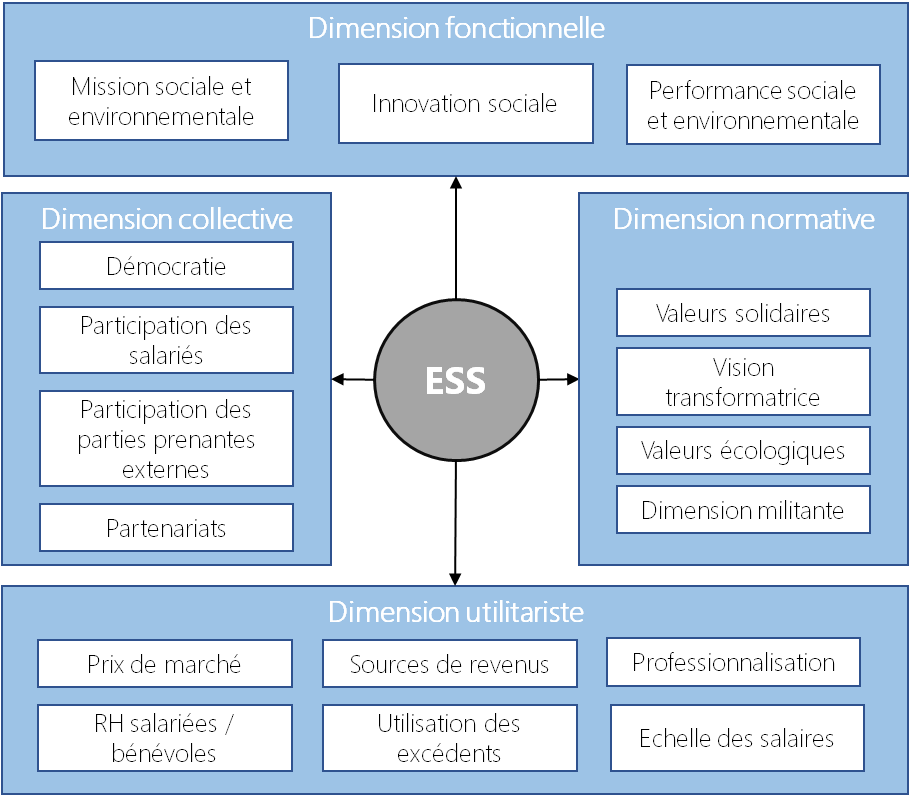
\includegraphics[width=\linewidth]{fig/dim_ess.png}
        \end{figure}

        \textbf{L'identité normative} fait écho au caractère \cit{social et solidaire} des \oess. Elle renvoie ainsi à la dimension socio-politique de l'ESS, par opposition à son rôle d'agent économique. \textcite[][p.293]{young2001organizational} parle d'une \citit{identité politique} qui vise à permettre la discussion et le débat, et éventuellement aboutir à une action collective.
        Malgré la forte hétérogénéité des organisations, le secteur pourrait ainsi se retrouver autour de valeurs ou de caractéristiques normatives. Une brève revue de littérature  de \textcite{mariaux2015leconomie} montre que l'\ess est présentée comme une économie différente, centrée sur l'humain, reposant sur la coopération entre les personnes et agissant pour l'intérêt général ou l'intérêt collectif et non pour des intérêts économiques ou personnels. \textcite{auger2014les} identifient des fondements normatifs importants dans des associations, comme la solidarité, la vie en communauté ou encore le respect. Mais elles soulignent que \citit{des valeurs plus austères sont évoquées}. \textcite{chedotel2004ambivalence} rappelle que cette vision peut être questionnée et qu'elle peut être vue comme un instrument de légitimation plutôt qu'une réelle identité de ses organisations. L'image d'entreprises responsables, agissant de manière éthique, aurait vocation à contrebalancer des scandales ou des cas de mauvaise gestion de structures de l'ESS. \\

       \textbf{L'identité utilitariste} s'inscrit dans l'approche gestionnaire de l'entreprise de l'ESS. \textcite{young2001organizational} la caractérise comme une \citit{identité économique}, qui traduit une volonté d'avoir un usage efficient des ressources au regard des objectifs à atteindre. \textcite[][p.840]{hansmann1980role} oppose ainsi des organisations \cit{commerciales} à des organisations reposant sur les dons (\citit{donative nonprofits}).
       L'identité utilitariste est adoptée par des organisations \citit{tournées vers le marché, orientées clients, auto-suffisantes, commerciales ou ayant une logique d’affaires} \parencite[][p. 414]{dart2004being}. Pour l'auteur, cette approche se caractérise par \citit{des objectifs exprimés en termes de générations de revenus, une organisation tournée vers le client, un fonctionnement managérial et une rhétorique commerciale} \parencite{dart2004legitimacy, mariaux2018leconomie}. Plusieurs auteurs observent et parfois s'inquiètent d'un mouvement généralisé de \cit{markétisation} ou de \cit{managérialisation}.  La tendance croissante des \eess à imiter le secteur lucratif \parencite{bidet2003insoutenable, valeau2013fonction} s'explique par une compétition croissante \parencite{dart2004being, frumkin2000when}, une volonté de légitimation (il est plus facile d'être reconnu lorsque l'on fait partie du système dominant et que l'on adopte ses codes) et une difficulté croissante à accéder aux financement dont ont besoin les organisations. En outre, il est intéressant de constater que l'approche de l'\ess par les valeurs (approche normative) - approche certes imparfaite, mais qui traçait une nette distinction avec le secteur lucratif - est progressivement remplacée par l'approche utilitariste, entrepreneuriale. Ainsi la loi cadre de 2014 caractérise l'\ess comme \citit{un mode d'entreprendre} \parencite{noauthor2014loi}, mettant ainsi en première place son rôle économique. \\

       Opérationnellement, l'identité utilitariste renvoie au mode de fonctionnement de l’entreprise : provenance des ressources (humaines et financières), adoption de prix de marché ou de prix adaptés à des situations spécifiques et possibilité de distribuer une partie des excédents. Ainsi, les entreprises ayant une forte identité utilitariste préfèrent le salariat au bénévolat et privilégient des ressources issues de leur activité à des dons et subventions. Elles déterminent les prix en fonction du marché et de la concurrence. A l'inverse, d'autres \oess proposent leurs produits gratuitement ou à moindre coût, ou au contraire à un prix plus élevé que le marché, mais considéré comme \cit{juste} (par exemple, les entreprises de commerce équitable). Enfin, certaines entreprises de l’\ess ont des statuts leur permettant de distribuer une partie des bénéfices réalisées. \\

        \textbf{L'identité fonctionnelle} de l'\ess ressort des travaux de \textcite{young2001organizational, young2000alternative} et \textcite{mariaux2018leconomie}. Les cas étudiés par \textcite[][p.292]{young2001organizational} mettent en lumière l'existence d'une identité qualifiée de \citit{goal-seeking systems} c'est-à-dire tournée avant tout vers la poursuite d'un but. Cette identité peut être rapprochée de l'analyse défendue par l'école de l'innovation sociale, pour qui l'efficacité sociale des \oess prime non seulement sur les aspects financiers mais aussi sur les valeurs \parencite{defourny2011approches}. Pour les auteurs, la question centrale est celle de l'utilité et l'innovation sociale \parencite{dees2003social}. Les questions gestionnaires ou normatives sont donc secondaires. Cependant, \textcite{auger2014les} soulignent le lien de cause à effet entre la dimension normative et la dimension fonctionnelle : ce sont souvent les valeurs personnelles, l'éthique et les convictions des managers qui façonnent la performance sociale et environnementale.  \\

        A notre connaissance, \textbf{la dimension collective} n'est pas identifiée comme une identité organisationnelle à proprement parler dans la littérature. Cependant, elle représente dans de nombreuses \oess un élément central et durable et constitue un caractère véritablement distinctif de l'ESS. Le critère de gouvernance démocratique, qui repose sur le principe \cit{une personne, une voix}, est ainsi inscrit dès l'article 1 de la loi de 2014 relative à l'ESS. Les statuts des organisations permettent d'intégrer à la gouvernance des parties prenantes multiples afin de mieux prendre en compte l'intérêt général dans les décisions. \textcite{petrella2014social} estiment par ailleurs que la place des entreprises sociales dans l'ESS dépend de leur capacité à s'organiser autour du caractère collectif et démocratique (p. 155). Une littérature abondante s'intéresse aux enjeux de la gestion du collectif dans les organisations de l'ESS, notamment du point de vue de la gouvernance et de l'intégration de multiples parties prenantes aux intérêts parfois convergents, parfois opposés. On peut ainsi distinguer des organisations \cit{mutuelles} (\citit{mutual nonprofit}), dont les dirigeants sont choisis par les membres et clients, et des organisations \cit{entrepreneuriales} dans lequelles la gouvernance fait l'objet d'un faible contrôle de la part des membres \parencite[][p.841]{hansmann1980role}. L'approche participative tient aussi une place importante dans la rhétorique des organisations, en particulier au sein des mouvements coopératifs et mutualistes qui sont nés d'une volonté d'agir en commun.
